\subsection{\label{sub:\projectname-AperB} \textsf{AperB}}

\paragraph{Símbol}

\begin{center} \bsfsymbol{AperB} \end{center}

\paragraph{Entrades i sortides}

% FIXME
No hi ha ports definits.

\paragraph{Funció}

% FIXME
Sense descripció.

\paragraph{Inespecificacions}

Cap.

\paragraph{Implementació}

\vhdlisting{AperB}

\begin{contendfig}
  \begin{center}
    \adjustbox{max width=\textwidth, max height=\textheight}{
      \bdfschematic{AperB}
    }
  \end{center}
  \caption{\label{fig:sch-\projectname-AperB} Esquemàtic per al bloc \textsf{AperB}}
\end{contendfig}

L'esquemàtic del bloc es pot veure a la figura~\ref{fig:sch-\projectname-AperB} (pàgina~\pageref{fig:sch-\projectname-AperB}).

% FIXME

\paragraph{Simulació}

\begin{contendfig}
  \begin{center}
    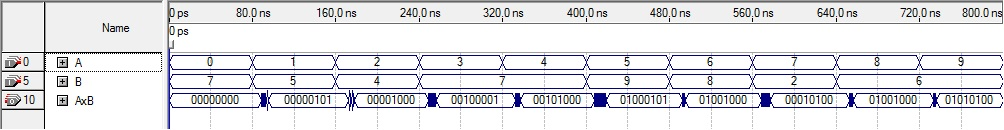
\includegraphics[scale=0.55]{../\projectname/assets/vwf/AperB.jpg}
  \end{center}
  \caption{\label{fig:sim-\projectname-AperB} Simulació per al bloc \textsf{AperB}}
\end{contendfig}

La simulació del bloc es pot veure a la figura~\ref{fig:sim-\projectname-AperB} (pàgina~\pageref{fig:sim-\projectname-AperB}).

% FIXME

\vspace{1cm}
